\documentclass[twoside]{book}

% Packages required by doxygen
\usepackage{fixltx2e}
\usepackage{calc}
\usepackage{doxygen}
\usepackage{graphicx}
\usepackage[utf8]{inputenc}
\usepackage{makeidx}
\usepackage{multicol}
\usepackage{multirow}
\PassOptionsToPackage{warn}{textcomp}
\usepackage{textcomp}
\usepackage[nointegrals]{wasysym}
\usepackage[table]{xcolor}

% Font selection
\usepackage[T1]{fontenc}
\usepackage{mathptmx}
\usepackage[scaled=.90]{helvet}
\usepackage{courier}
\usepackage{amssymb}
\usepackage{sectsty}
\renewcommand{\familydefault}{\sfdefault}
\allsectionsfont{%
  \fontseries{bc}\selectfont%
  \color{darkgray}%
}
\renewcommand{\DoxyLabelFont}{%
  \fontseries{bc}\selectfont%
  \color{darkgray}%
}
\newcommand{\+}{\discretionary{\mbox{\scriptsize$\hookleftarrow$}}{}{}}

% Page & text layout
\usepackage{geometry}
\geometry{%
  a4paper,%
  top=2.5cm,%
  bottom=2.5cm,%
  left=2.5cm,%
  right=2.5cm%
}
\tolerance=750
\hfuzz=15pt
\hbadness=750
\setlength{\emergencystretch}{15pt}
\setlength{\parindent}{0cm}
\setlength{\parskip}{0.2cm}
\makeatletter
\renewcommand{\paragraph}{%
  \@startsection{paragraph}{4}{0ex}{-1.0ex}{1.0ex}{%
    \normalfont\normalsize\bfseries\SS@parafont%
  }%
}
\renewcommand{\subparagraph}{%
  \@startsection{subparagraph}{5}{0ex}{-1.0ex}{1.0ex}{%
    \normalfont\normalsize\bfseries\SS@subparafont%
  }%
}
\makeatother

% Headers & footers
\usepackage{fancyhdr}
\pagestyle{fancyplain}
\fancyhead[LE]{\fancyplain{}{\bfseries\thepage}}
\fancyhead[CE]{\fancyplain{}{}}
\fancyhead[RE]{\fancyplain{}{\bfseries\leftmark}}
\fancyhead[LO]{\fancyplain{}{\bfseries\rightmark}}
\fancyhead[CO]{\fancyplain{}{}}
\fancyhead[RO]{\fancyplain{}{\bfseries\thepage}}
\fancyfoot[LE]{\fancyplain{}{}}
\fancyfoot[CE]{\fancyplain{}{}}
\fancyfoot[RE]{\fancyplain{}{\bfseries\scriptsize Generated on Fri Nov 21 2014 23\+:30\+:33 for Jamie Slowgrove -\/ P\+G\+G Assignment 1 -\/ S\+D\+L by Doxygen }}
\fancyfoot[LO]{\fancyplain{}{\bfseries\scriptsize Generated on Fri Nov 21 2014 23\+:30\+:33 for Jamie Slowgrove -\/ P\+G\+G Assignment 1 -\/ S\+D\+L by Doxygen }}
\fancyfoot[CO]{\fancyplain{}{}}
\fancyfoot[RO]{\fancyplain{}{}}
\renewcommand{\footrulewidth}{0.4pt}
\renewcommand{\chaptermark}[1]{%
  \markboth{#1}{}%
}
\renewcommand{\sectionmark}[1]{%
  \markright{\thesection\ #1}%
}

% Indices & bibliography
\usepackage{natbib}
\usepackage[titles]{tocloft}
\setcounter{tocdepth}{3}
\setcounter{secnumdepth}{5}
\makeindex

% Hyperlinks (required, but should be loaded last)
\usepackage{ifpdf}
\ifpdf
  \usepackage[pdftex,pagebackref=true]{hyperref}
\else
  \usepackage[ps2pdf,pagebackref=true]{hyperref}
\fi
\hypersetup{%
  colorlinks=true,%
  linkcolor=blue,%
  citecolor=blue,%
  unicode%
}

% Custom commands
\newcommand{\clearemptydoublepage}{%
  \newpage{\pagestyle{empty}\cleardoublepage}%
}


%===== C O N T E N T S =====

\begin{document}

% Titlepage & ToC
\hypersetup{pageanchor=false,
             bookmarks=true,
             bookmarksnumbered=true,
             pdfencoding=unicode
            }
\pagenumbering{roman}
\begin{titlepage}
\vspace*{7cm}
\begin{center}%
{\Large Jamie Slowgrove -\/ P\+G\+G Assignment 1 -\/ S\+D\+L }\\
\vspace*{1cm}
{\large Generated by Doxygen 1.8.8}\\
\vspace*{0.5cm}
{\small Fri Nov 21 2014 23:30:33}\\
\end{center}
\end{titlepage}
\clearemptydoublepage
\tableofcontents
\clearemptydoublepage
\pagenumbering{arabic}
\hypersetup{pageanchor=true}

%--- Begin generated contents ---
\chapter{Class Index}
\section{Class List}
Here are the classes, structs, unions and interfaces with brief descriptions\+:\begin{DoxyCompactList}
\item\contentsline{section}{\hyperlink{class_building}{Building} \\*Creates a \hyperlink{class_building}{Building} object that inherits \hyperlink{class_entity}{Entity} }{\pageref{class_building}}{}
\item\contentsline{section}{\hyperlink{class_entity}{Entity} \\*Creates an \hyperlink{class_entity}{Entity} object Creates an \hyperlink{class_entity}{Entity} object with a \hyperlink{class_texture}{Texture} (including variables for the source and destination dimensions) and position }{\pageref{class_entity}}{}
\item\contentsline{section}{\hyperlink{class_minion}{Minion} \\*Creates a \hyperlink{class_minion}{Minion} object that inherits \hyperlink{class_entity}{Entity} }{\pageref{class_minion}}{}
\item\contentsline{section}{\hyperlink{class_player}{Player} \\*Creates a \hyperlink{class_player}{Player} object }{\pageref{class_player}}{}
\item\contentsline{section}{\hyperlink{class_texture}{Texture} \\*Creates a \hyperlink{class_texture}{Texture} for use with a renderer Creates a \hyperlink{class_texture}{Texture} from an image file, this can then be used with a renderer }{\pageref{class_texture}}{}
\item\contentsline{section}{\hyperlink{class_turret}{Turret} \\*Creates a \hyperlink{class_turret}{Turret} object that inherits \hyperlink{class_entity}{Entity} }{\pageref{class_turret}}{}
\end{DoxyCompactList}

\chapter{Class Documentation}
\hypertarget{class_texture}{\section{Texture Class Reference}
\label{class_texture}\index{Texture@{Texture}}
}


Creates a \hyperlink{class_texture}{Texture} for use with a renderer Creates a \hyperlink{class_texture}{Texture} from an image file, this can then be used with a renderer.  




{\ttfamily \#include $<$texture.\+h$>$}



Collaboration diagram for Texture\+:
\nopagebreak
\begin{figure}[H]
\begin{center}
\leavevmode
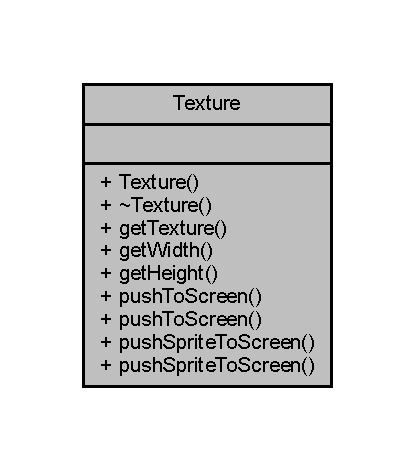
\includegraphics[width=199pt]{class_texture__coll__graph}
\end{center}
\end{figure}
\subsection*{Public Member Functions}
\begin{DoxyCompactItemize}
\item 
\hyperlink{class_texture_a6edf59e3b10e474356e8a7878af56b83}{Texture} (std\+::string, S\+D\+L\+\_\+\+Renderer $\ast$, bool)
\item 
\hyperlink{class_texture_a09c4bcb7462f64c1d20fa69dba3cee8a}{$\sim$\+Texture} ()
\item 
S\+D\+L\+\_\+\+Texture $\ast$ \hyperlink{class_texture_a77a1ae0043a4b318a60df3b02ef2d3f6}{get\+Texture} ()
\item 
int \hyperlink{class_texture_a91a6fd3355bc870194851514194daaab}{get\+Width} ()
\item 
int \hyperlink{class_texture_a80e143905655b173df5994300088ce35}{get\+Height} ()
\item 
void \hyperlink{class_texture_aec498f1f84eb10bb60d3c3117884e70f}{push\+To\+Screen} (S\+D\+L\+\_\+\+Renderer $\ast$, int, int)
\item 
void \hyperlink{class_texture_ab3b1f6aa29a50ef2c012fbc9d0cb8bd8}{push\+To\+Screen} (S\+D\+L\+\_\+\+Renderer $\ast$, int, int, int, int)
\item 
void \hyperlink{class_texture_a703db8963b46b751b8affce1807725b7}{push\+Sprite\+To\+Screen} (S\+D\+L\+\_\+\+Renderer $\ast$, int, int, int, int, int, int)
\item 
void \hyperlink{class_texture_a105a3aba66afb7d223ac086aa465b70d}{push\+Sprite\+To\+Screen} (S\+D\+L\+\_\+\+Renderer $\ast$, int, int, int, int, int, int, int, int)
\end{DoxyCompactItemize}


\subsection{Detailed Description}
Creates a \hyperlink{class_texture}{Texture} for use with a renderer Creates a \hyperlink{class_texture}{Texture} from an image file, this can then be used with a renderer. 

\subsection{Constructor \& Destructor Documentation}
\hypertarget{class_texture_a6edf59e3b10e474356e8a7878af56b83}{\index{Texture@{Texture}!Texture@{Texture}}
\index{Texture@{Texture}!Texture@{Texture}}
\subsubsection[{Texture}]{\setlength{\rightskip}{0pt plus 5cm}Texture\+::\+Texture (
\begin{DoxyParamCaption}
\item[{std\+::string}]{file\+Name, }
\item[{S\+D\+L\+\_\+\+Renderer $\ast$}]{renderer, }
\item[{bool}]{magenta\+Alpha}
\end{DoxyParamCaption}
)}}\label{class_texture_a6edf59e3b10e474356e8a7878af56b83}
Constructs a \hyperlink{class_texture}{Texture} Creates a \hyperlink{class_texture}{Texture} using an image location and a renderer. The magenta pixels of this image can represent alpha if needed. 
\begin{DoxyParams}{Parameters}
{\em std\+::string} & The location of the image file. \\
\hline
{\em S\+D\+L\+\_\+\+Renderer$\ast$} & The renderer. \\
\hline
{\em bool} & If true any magenta pixels in the image will be converted to alpha \\
\hline
\end{DoxyParams}
\hypertarget{class_texture_a09c4bcb7462f64c1d20fa69dba3cee8a}{\index{Texture@{Texture}!````~Texture@{$\sim$\+Texture}}
\index{````~Texture@{$\sim$\+Texture}!Texture@{Texture}}
\subsubsection[{$\sim$\+Texture}]{\setlength{\rightskip}{0pt plus 5cm}Texture\+::$\sim$\+Texture (
\begin{DoxyParamCaption}
{}
\end{DoxyParamCaption}
)}}\label{class_texture_a09c4bcb7462f64c1d20fa69dba3cee8a}
De-\/constructs a \hyperlink{class_texture}{Texture} De-\/constructs the \hyperlink{class_texture}{Texture} deleting the \hyperlink{class_texture}{Texture} from memory. 

\subsection{Member Function Documentation}
\hypertarget{class_texture_a80e143905655b173df5994300088ce35}{\index{Texture@{Texture}!get\+Height@{get\+Height}}
\index{get\+Height@{get\+Height}!Texture@{Texture}}
\subsubsection[{get\+Height}]{\setlength{\rightskip}{0pt plus 5cm}int Texture\+::get\+Height (
\begin{DoxyParamCaption}
{}
\end{DoxyParamCaption}
)}}\label{class_texture_a80e143905655b173df5994300088ce35}
Getter \# Returns texture\+Height \begin{DoxyReturn}{Returns}
the value of texture\+Height. 
\end{DoxyReturn}
\hypertarget{class_texture_a77a1ae0043a4b318a60df3b02ef2d3f6}{\index{Texture@{Texture}!get\+Texture@{get\+Texture}}
\index{get\+Texture@{get\+Texture}!Texture@{Texture}}
\subsubsection[{get\+Texture}]{\setlength{\rightskip}{0pt plus 5cm}S\+D\+L\+\_\+\+Texture $\ast$ Texture\+::get\+Texture (
\begin{DoxyParamCaption}
{}
\end{DoxyParamCaption}
)}}\label{class_texture_a77a1ae0043a4b318a60df3b02ef2d3f6}
Getter \# Returns a pointer to the \hyperlink{class_texture}{Texture} \begin{DoxyReturn}{Returns}
a pointer to the \hyperlink{class_texture}{Texture} data. 
\end{DoxyReturn}
\hypertarget{class_texture_a91a6fd3355bc870194851514194daaab}{\index{Texture@{Texture}!get\+Width@{get\+Width}}
\index{get\+Width@{get\+Width}!Texture@{Texture}}
\subsubsection[{get\+Width}]{\setlength{\rightskip}{0pt plus 5cm}int Texture\+::get\+Width (
\begin{DoxyParamCaption}
{}
\end{DoxyParamCaption}
)}}\label{class_texture_a91a6fd3355bc870194851514194daaab}
Getter \# Returns texture\+Width \begin{DoxyReturn}{Returns}
the value of texture\+Width. 
\end{DoxyReturn}
\hypertarget{class_texture_a703db8963b46b751b8affce1807725b7}{\index{Texture@{Texture}!push\+Sprite\+To\+Screen@{push\+Sprite\+To\+Screen}}
\index{push\+Sprite\+To\+Screen@{push\+Sprite\+To\+Screen}!Texture@{Texture}}
\subsubsection[{push\+Sprite\+To\+Screen}]{\setlength{\rightskip}{0pt plus 5cm}void Texture\+::push\+Sprite\+To\+Screen (
\begin{DoxyParamCaption}
\item[{S\+D\+L\+\_\+\+Renderer $\ast$}]{renderer, }
\item[{int}]{x, }
\item[{int}]{y, }
\item[{int}]{src\+X, }
\item[{int}]{src\+Y, }
\item[{int}]{src\+Width, }
\item[{int}]{src\+Height}
\end{DoxyParamCaption}
)}}\label{class_texture_a703db8963b46b751b8affce1807725b7}
Pushes the image to the Renderer, to the X\+Y Coordinates. Only displays the source rectangle inputed. 
\begin{DoxyParams}{Parameters}
{\em S\+D\+L\+\_\+\+Renderer$\ast$} & The renderer. \\
\hline
{\em int} & x coordinate of the image. \\
\hline
{\em int} & y coordinate of the image. \\
\hline
{\em int} & x coordinate of the source image. \\
\hline
{\em int} & y coordinate of the source image. \\
\hline
{\em int} & width of the source image. \\
\hline
{\em int} & height of the source image. \\
\hline
\end{DoxyParams}


Here is the caller graph for this function\+:
\nopagebreak
\begin{figure}[H]
\begin{center}
\leavevmode
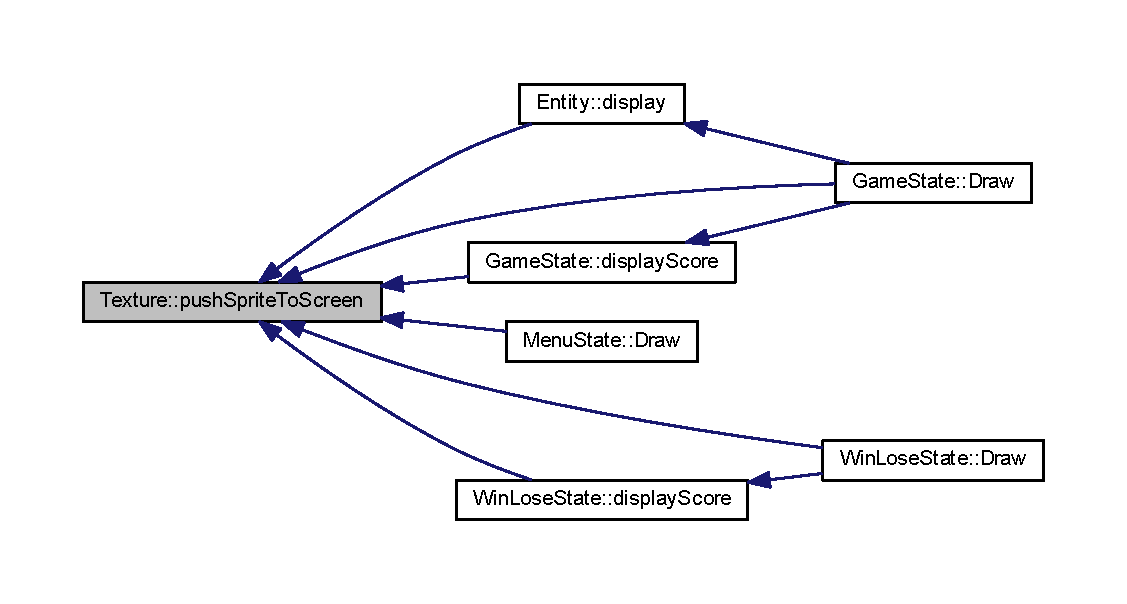
\includegraphics[width=350pt]{class_texture_a703db8963b46b751b8affce1807725b7_icgraph}
\end{center}
\end{figure}


\hypertarget{class_texture_a105a3aba66afb7d223ac086aa465b70d}{\index{Texture@{Texture}!push\+Sprite\+To\+Screen@{push\+Sprite\+To\+Screen}}
\index{push\+Sprite\+To\+Screen@{push\+Sprite\+To\+Screen}!Texture@{Texture}}
\subsubsection[{push\+Sprite\+To\+Screen}]{\setlength{\rightskip}{0pt plus 5cm}void Texture\+::push\+Sprite\+To\+Screen (
\begin{DoxyParamCaption}
\item[{S\+D\+L\+\_\+\+Renderer $\ast$}]{renderer, }
\item[{int}]{x, }
\item[{int}]{y, }
\item[{int}]{src\+X, }
\item[{int}]{src\+Y, }
\item[{int}]{src\+Width, }
\item[{int}]{src\+Height, }
\item[{int}]{width, }
\item[{int}]{height}
\end{DoxyParamCaption}
)}}\label{class_texture_a105a3aba66afb7d223ac086aa465b70d}
Pushes the image to the Renderer, to the X\+Y Coordinates. Only displays the source rectangle inputed. This is scaled to the width and height inputed. 
\begin{DoxyParams}{Parameters}
{\em S\+D\+L\+\_\+\+Renderer$\ast$} & The renderer. \\
\hline
{\em int} & x coordinate of the image. \\
\hline
{\em int} & y coordinate of the image. \\
\hline
{\em int} & x coordinate of the source image. \\
\hline
{\em int} & y coordinate of the source image. \\
\hline
{\em int} & width of the source image. \\
\hline
{\em int} & height of the source image. \\
\hline
{\em int} & width of the scaled image. \\
\hline
{\em int} & height of the scaled image. \\
\hline
\end{DoxyParams}
\hypertarget{class_texture_aec498f1f84eb10bb60d3c3117884e70f}{\index{Texture@{Texture}!push\+To\+Screen@{push\+To\+Screen}}
\index{push\+To\+Screen@{push\+To\+Screen}!Texture@{Texture}}
\subsubsection[{push\+To\+Screen}]{\setlength{\rightskip}{0pt plus 5cm}void Texture\+::push\+To\+Screen (
\begin{DoxyParamCaption}
\item[{S\+D\+L\+\_\+\+Renderer $\ast$}]{renderer, }
\item[{int}]{x, }
\item[{int}]{y}
\end{DoxyParamCaption}
)}}\label{class_texture_aec498f1f84eb10bb60d3c3117884e70f}
Pushes the image to the Renderer, to the X\+Y Coordinates. 
\begin{DoxyParams}{Parameters}
{\em S\+D\+L\+\_\+\+Renderer$\ast$} & The renderer. \\
\hline
{\em int} & x coordinate of the image. \\
\hline
{\em int} & y coordinate of the image. \\
\hline
\end{DoxyParams}


Here is the caller graph for this function\+:
\nopagebreak
\begin{figure}[H]
\begin{center}
\leavevmode
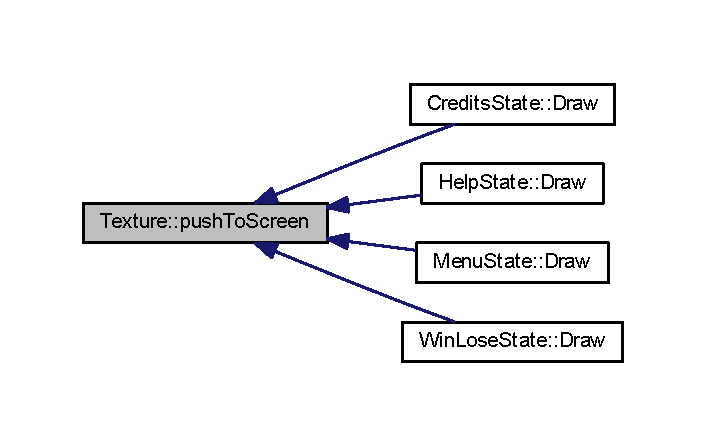
\includegraphics[width=339pt]{class_texture_aec498f1f84eb10bb60d3c3117884e70f_icgraph}
\end{center}
\end{figure}


\hypertarget{class_texture_ab3b1f6aa29a50ef2c012fbc9d0cb8bd8}{\index{Texture@{Texture}!push\+To\+Screen@{push\+To\+Screen}}
\index{push\+To\+Screen@{push\+To\+Screen}!Texture@{Texture}}
\subsubsection[{push\+To\+Screen}]{\setlength{\rightskip}{0pt plus 5cm}void Texture\+::push\+To\+Screen (
\begin{DoxyParamCaption}
\item[{S\+D\+L\+\_\+\+Renderer $\ast$}]{renderer, }
\item[{int}]{x, }
\item[{int}]{y, }
\item[{int}]{width, }
\item[{int}]{height}
\end{DoxyParamCaption}
)}}\label{class_texture_ab3b1f6aa29a50ef2c012fbc9d0cb8bd8}
Pushes the image to the Renderer, to the X\+Y Coordinates. This is scaled to the width and height inputed. 
\begin{DoxyParams}{Parameters}
{\em S\+D\+L\+\_\+\+Renderer$\ast$} & The renderer. \\
\hline
{\em int} & x coordinate of the image. \\
\hline
{\em int} & y coordinate of the image. \\
\hline
{\em int} & width of the scaled image. \\
\hline
{\em int} & height of the scaled image. \\
\hline
\end{DoxyParams}


The documentation for this class was generated from the following files\+:\begin{DoxyCompactItemize}
\item 
P\+G\+G\+Assignment1\+S\+D\+L/texture.\+h\item 
P\+G\+G\+Assignment1\+S\+D\+L/texture.\+cpp\end{DoxyCompactItemize}

%--- End generated contents ---

% Index
\newpage
\phantomsection
\addcontentsline{toc}{chapter}{Index}
\printindex

\end{document}
